\begin{algorithm}[t]
\begin{algorithmic}[1]
\caption{Алгоритм ослабленного синтаксического анализа регулярной аппроксимации динамически формируемого выражения}
\label{parsing}
\Function{parse}{$grammar, automaton$}
  \State{$inputGraph \gets$ construct inner graph}
  \State{   representation of $automaton$}
  \State{$parserSource \gets$ generate RNGLR parse tables for $grammar$}
  \If{$inputGraph$ contains no edges}
    \If{$parserSource$ accepts empty input} {report success}
    \Else { report failure}
    \EndIf
  \Else
    \State{\Call{addVertex}{$inputGraph.startVertex, startState$}}
    \State{$\mathcal{Q}.Enqueue(inputGraph.startVertex)$}
    \While{$Q$ is not empty}
      \State{$v \gets \mathcal{Q}.Dequeue()$}
      \State{\Call{makeReductions}{$v$}}
      \State{\Call{push}{$v$}}
      \State{\Call{applyPassingReductions}{$v$}}
    \EndWhile
    \If{$\exists v_f: v_f.level = q_f$ and\par
\hskip1cm $v_f.state$ is accepting} {report success}
    \Else { report failure}
    \EndIf
  \EndIf
\EndFunction
\end{algorithmic}
\end{algorithm}

\begin{algorithm}
\begin{algorithmic}[1]
\caption{Обработка вершины внутреннего графа}
\label{processVertex}
\Function{push}{$innerGraphV$}
  \State{$\mathcal{U} \gets$ copy $innerGraphV.unprocessed$}
  \State{clear $innerGraphV.unprocessed$}
  \ForAll{$v_{h}\gets\mathcal{U}$}  
    \ForAll{$e\gets\mbox{ outgoing edges of }innerGraphV$}
      \State{$push \gets$ calculate next state by $v_{h}.state$ and}
      \State{    the token on $e$}
      \State{\Call{addEdge}{$v_{h}, e.Head, push, false$}}
      \State{add $v_{h}$ in $innerGraphV.processed$}
    \EndFor
  \EndFor
\EndFunction

\Function{makeReductions}{$innerGraphV$}
  \While{$innerGraphV.reductions$ is not empty}
    \State{$(startV, N, l) \gets innerGraphV.reductions.Dequeue()$}
    \State{find the set of vertices $\mathcal{X}$ reachable from $startV$}
    \State{    along the path of length ($l-1$), or $0$ if $l=0$;}
    \State{add $(startV, N, l-i)$ in $v.passingReductions$,}
    \State{    where $v$ is an $i$-th vertex of the path}
    \ForAll{$v_{h}\gets\mathcal{X}$}
      \State{$state_{t} \gets$ calculate new state by $v_{h}.state$ and}
      \State{    nonterminal $N$}
      \State{\Call{addEdge}{$v_{h}, startV, state_{t}, (l=0)$}}
    \EndFor
  \EndWhile
\EndFunction

\Function{applyPassingReductions}{$G$}
  \ForAll{$(v, edge) \gets G.passingReductionsToHandle$}
    \ForAll{$(startV, N, l) \gets v.passingReductions.Dequeue()$}
      \State{find the set of vertices $\mathcal{X}$,}
      \State{    reachable from $edge$ along the path of length ($l-1$)}
      \ForAll{$v_{h}\gets\mathcal{X}$}
        \State{$state_{t} \gets$ calculate new state by $v_{h}.state$ and}
        \State{    nonterminal $N$}
        \State{\Call{addEdge}{$v_{h}, startV, state_{t}, false$}}
      \EndFor
    \EndFor
  \EndFor
\EndFunction
\end{algorithmic}
\end{algorithm}

\section{Алгоритм ослабленного синтаксического анализа регулярной аппроксимации динамически формируемого выражения}

\subsection{Описание алгоритма}
Алгоритм принимает на вход эталонную грамматику $G$ над алфавитом терминальных символов $T$ и детерминированный конечный автомат $(Q,\Sigma,\delta,q_0,q_f)$, имеющий одно стартовое состояние $q_0$, одно конечное состояние $q_f$, без $\epsilon$-переходов, где $\Sigma \subseteq T$~--- алфавит входных символов, $Q$~--- множество состояний, $\delta$~--- отношение перехода. По описанию  грамматики генерируются управляющие RNGLR-таблицы и некоторая вспомогательная информация (называемая $parserSource$ в псевдокоде).

Алгоритм производит обход графа входного автомата и последовательно строит GSS тем же способом, как это делает RNGLR-алгоритм. Однако, так как мы имеем дело с графом вместо линейного потока, понятие следующего символа трансформируется во \emph{множество терминальных символов}, лежащих на всех исходящих рёбрах данной вершины, что несколько изменяет операции shift и reduce (смотри строку 5 в алгоритме~\ref{processVertex} и строки 9 и 21 в алгоритме~\ref{gss_construction}). Для того, чтобы управлять порядком обработки вершин входного графа, мы используем глобальную очередь $\mathcal{Q}$. Каждый раз, когда добавляется новая вершина GSS, сначала необходимо произвести все свёртки длины 0, после чего выполнить сдвиг следующих токенов со входа. Таким образом необходимо добавить соответствующую вершину графа в очередь на обработку. Добавление нового ребра GSS может порождать новые свёртки, таким образом в очередь на обработку необходимо добавить вершину входного графа, которой соответствует начальная вершина добавленного ребра. Детальное описание процесса построения GSS приведено в алгоритме~\ref{parsing}. Свёртки производятся вдоль путей в GSS, и если было добавлено ребро, начальная вершина которого ранее присутствовала в GSS, необходимо заново вычислить проходящие через эту вершину свёртки (смотри функцию applyPassingReductions в алгоритме~\ref{processVertex}).


Так же как и RNGLR, мы ассоциируем вершины GSS с позициями входного графа, однако в нашем случае уровень вершины~--- это состояние входного автомата. Мы строим внутреннюю структуру данных (в дальнейшем изложении называемую \emph{внутренним графом}) посредством копирования графа входного автомата и ассоциации с его вершинами следующих коллекций.
\begin{itemize}
  \item \emph{processed}: вершины GSS, для которых ранее были вычислены все операции push. Это множество агрегирует все вершины GSS, ассоциированные с вершиной внутреннего графа.
  \item \emph{unprocessed}: вершины GSS, операции push для которых ещё только предстоит выполнить. Это множество аналогично множеству $\mathcal{Q}$ алгоритма RNGLR.
  \item \emph{reductions}: очередь, аналогичная очереди $\mathcal{R}$ RNGLR-алгоритма: все операции reduce, которые ещё только предстоит выполнить.
  \item \emph{passingReductionsToHandle}: пары из вершины GSS и ребра GSS, вдоль которых необходимо осуществлять проходящие свёртки.
\end{itemize}

\begin{algorithm}[H]
\begin{algorithmic}[1]
\caption{Построение GSS}
\label{gss_construction}
\Function{addVertex}{$innerGraphV, state$}
  \State{$v \gets$ find a vertex with state $=state$ in}
  \State{    $innerGraphV.processed \cup innerGraphV.unprocessed$}
  \If{$v$ is not $null$ } \Comment{Вершина была найдена в GSS}
    \State{\Return{($v, false$)}} 
  \Else
    \State{$v \gets$ create new vertex for $innerGraphV$ with state $state$}
    \State{add $v$ in $innerGraphV.unprocessed$}
    \ForAll{$e\gets\mbox{ outgoing edges of }innerGraphV$}
      \State{calculate the set of zero-reductions by $v$}
      \State{    and the token on $e$ and}
      \State{    add them in $innerGraphV.reductions$}
    \EndFor
    \State{\Return{$(v, true$)}}
  \EndIf
\EndFunction

\Function{addEdge}{$v_{h}, innerGraphV, state_{t}, isZeroReduction$}
  \State{$(v_{t}, isNew) \gets$ \Call{addVertex}{$innerGraphV, state_{t}$}}
  \If{GSS does not contain edge from $v_{t}$ to $v_{h}$}
    \State{$edge \gets$ create new edge from $v_{t}$ to $v_{h}$}
    \State{$\mathcal{Q}.Enqueue(innerGraphV)$}
    \If{not $isNew$ and $v_{t}.passingReductions.Count>0$}
      \State{add $(v_{t}, edge)$ in $innerGraphV.passingReductionsToHandle$}
    \EndIf
    \If{not $isZeroReduction$}
      \ForAll{$e\gets\mbox{ in outgoing edges of }innerGraphV$}
        \State{calculate the set of reductions by $v$}
        \State{    and the token on $e$ and}
        \State{    add them in $innerGraphV.reductions$}
      \EndFor
    \EndIf
  \EndIf
\EndFunction
\end{algorithmic}
\end{algorithm}

Помимо состояния анализатора $state$ и уровня $level$ (который совпадает с состоянием входного автомата), в вершине GSS хранится коллекция \emph{проходящих свёрток}. Проходящая свёртка~--- это тройка $(startV, N, l)$, соответствующая свёртке, чей путь содержит данную вершину GSS. Аналогичная тройка используется в RNGLR-алгоритме для описания свёртки, но в данном случае $l$ обозначает длину оставшейся части пути. Проходящие свёртки сохраняются в каждой вершине пути (кроме первой и последней) во время поиска путей в функции $makeReductions$ (см. алгоритм~\ref{processVertex}).

\subsection{Построение компактного представления леса разбора}
В качестве компактного представления леса разбора всех корректных выражений из множества значений динамически формируемого выражения используется граф SPPF. Построение компактного представления осуществляется одновременно с синтаксическим разбором во время построения графа стеков GSS, также как и в алгоритме RNGLR.

С каждым ребром GSS ассоциируется список лесов разбора фрагмента выражения. В графе GSS нет кратных рёбер, поэтому если во время работы функции \emph{addEdge} в нем было найдено добавляемое ребро, то с ним ассоциируется новый лес разбора, при этом в очередь на обработку не добавляется никаких вершин входного графа.  

При добавлении в GSS ребра, соответствующего считанной со входа лексеме, создаётся (и ассоциируется с ним) граф из одной терминальной вершины. Так как входной автомат является детерминированным, с ребром GSS ассоциируется не более одного такого графа.

При обработке свёртки алгоритм осуществляет поиск всех путей в графе GSS заданной длины, после чего происходит добавление в GSS новых рёбер, соответствующих данной свёртке. С каждым таким ребром ассоциируется лес, имеющий в качестве корня (вершины, у которой нет входных рёбер) вершину, соответствующую нетерминалу, к которому осуществлялась свёртка. Ребра каждого из найденных путей, перечисленные в обратном порядке, образуют правую часть некоторого правила грамматики, по которому осуществляется свёртка. Для каждого пути создаётся вершина, помеченная номером такого правила, и добавляется в лес как непосредственно достижимая из корня. Каждое ребро пути ассоциировано со списком лесов вывода символа из правой части правила. Непосредственно достижимыми вершинами вершины-правила становятся ссылки на такие списки, за счёт чего осуществляется переиспользование фрагментов леса.

В алгоритме RNGLR наличие нескольких путей, вдоль которых осуществляется свёртка к нетерминалу, означает существование более чем одного варианта вывода нетерминала. В нашем случае данная ситуация соответствует различным фрагментам нескольких выражений из входного регулярного множества, которые сворачиваются к одному нетерминалу. 

В конце работы алгоритма осуществляется поиск рёбер GSS, для каждого из которых верно, что конечная вершина имеет уровень, равный финальному состоянию входного автомата, и принимающее состояние (accepting state). Результирующее представление леса разбора получается путём удаления недостижимых вершин из графа, созданного объединением лесов разбора, ассоциированных с найденными рёбрами GSS.

Рассмотрим следующий фрагмент кода, динамически формирующий выражение \emph{expr} в строке 4. 
\begin{verbatim}
1 string expr = "" ;
2 for(int i = 0; i < len; i++) 
3 {
4     expr = "()" + expr;
5 }
\end{verbatim}

Множество значений выражения \emph{expr} аппроксимируется регулярным выражением $(\mbox{\texttt{LBR }} \mbox{\texttt{RBR}})*$, где $\mbox{\texttt{LBR }}$ соответствует открывающейся скобке, а $\mbox{\texttt{RBR}}$~--- закрывающейся. Граф конечного автомата, задающего такую аппроксимацию, изображён на рис.~\ref{input}.
\begin{figure}[!h]
 \centering
 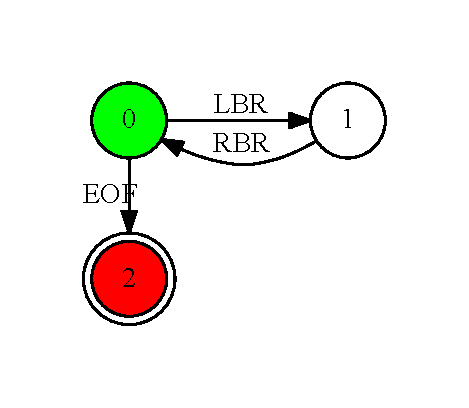
\includegraphics[width=3cm]{Verbitskaya/pics/input.pdf}
 \caption{Конечный автомат, задающий регулярную аппроксимацию выражения \emph{expr}}
 \label{input}
\end{figure}

В результате работы предложенного алгоритма будет получено конечное представление леса разбора SPPF, изображённое на рис.~\ref{sppf}.
\begin{figure}[!h]
 \centering
 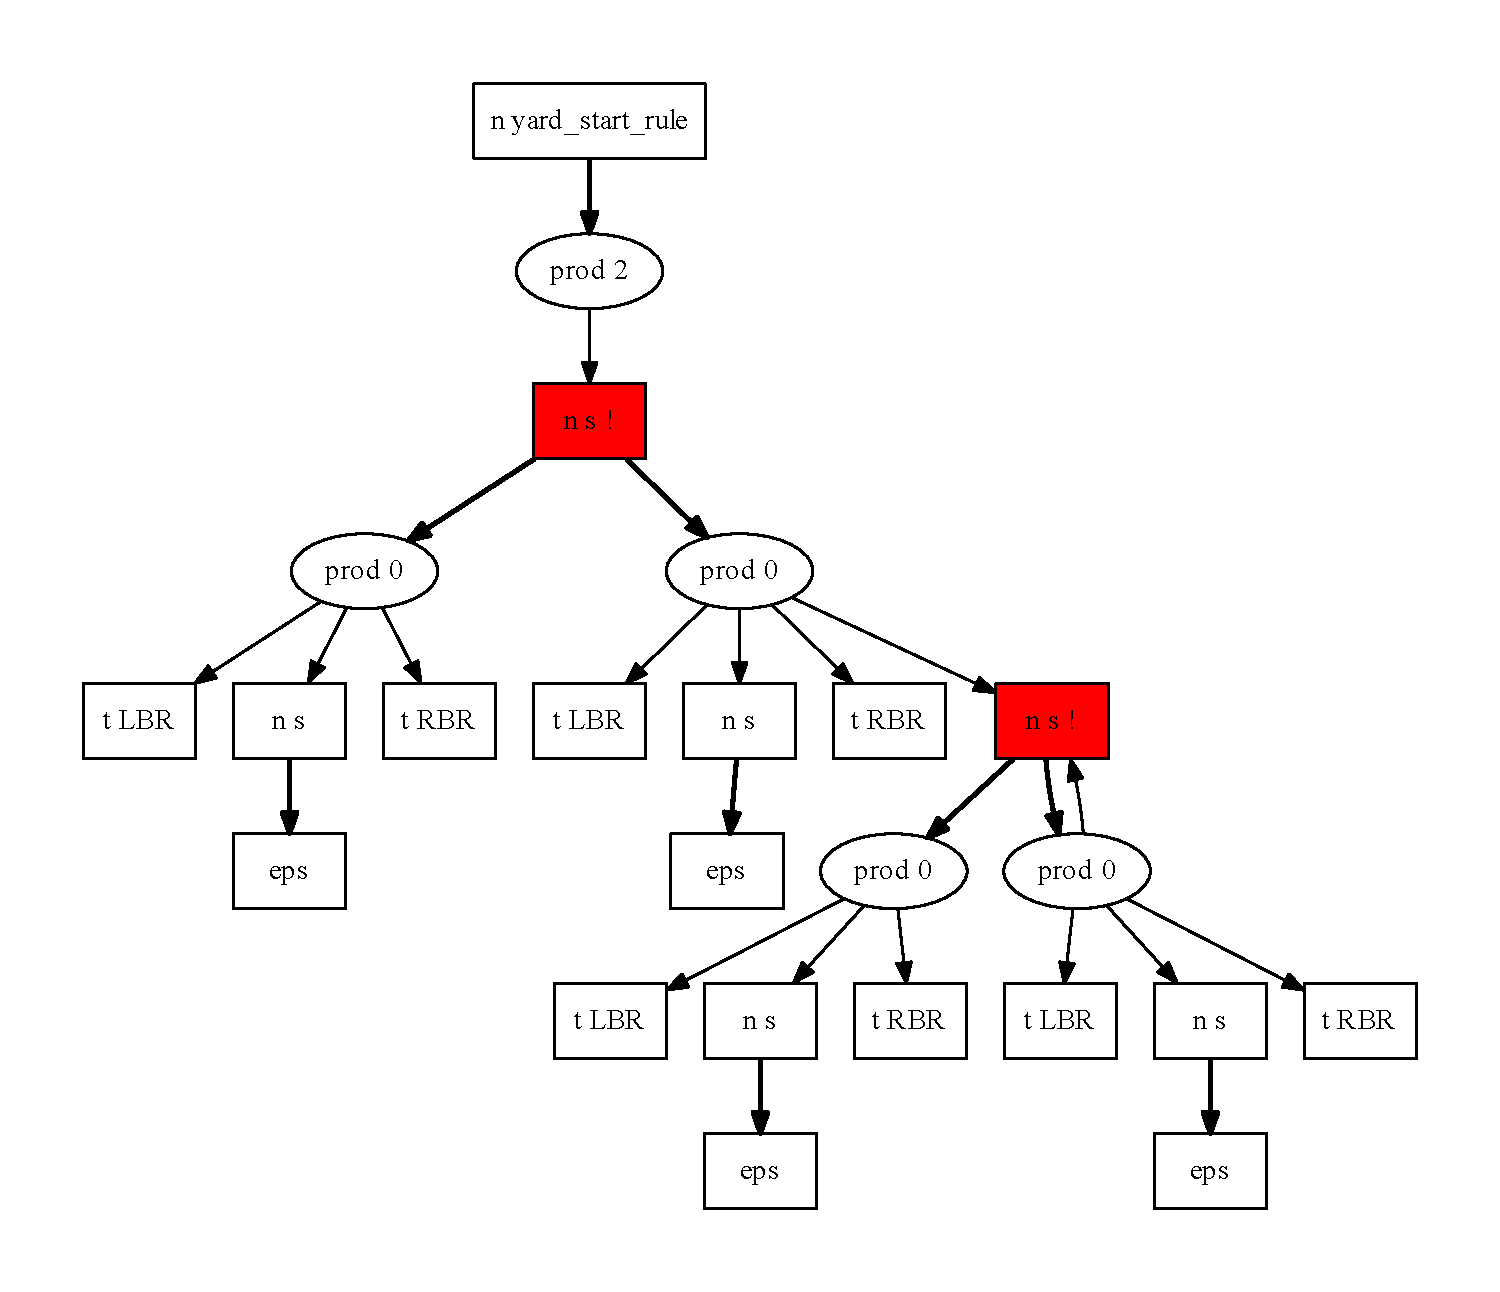
\includegraphics[width=\textwidth]{Verbitskaya/pics/sppf.pdf}
 \caption{Конечное представление леса разбора для выражения \emph{expr}}
 \label{sppf}
\end{figure}

%\begin{figure}[!h]
% \centering
% 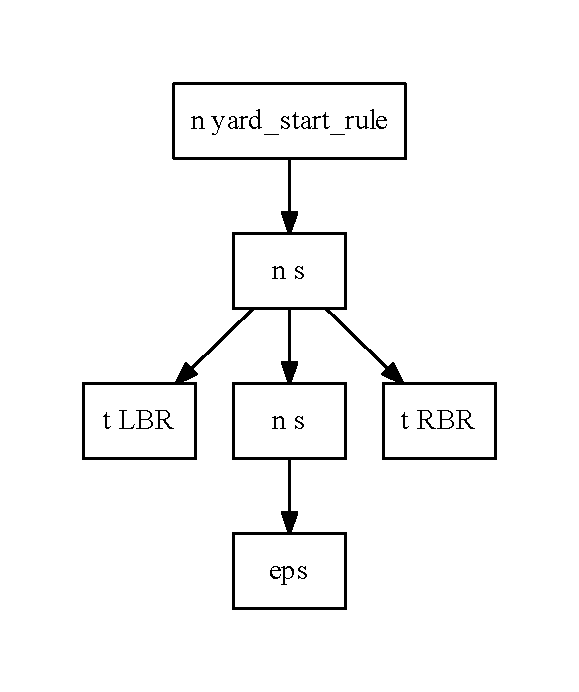
\includegraphics[]{pics/sppf1.pdf}
% \caption{Дерево вывода для выражения $expr="()"$}
% \label{sppf1}
%\end{figure}
%\begin{figure}[!h]
% \centering
% 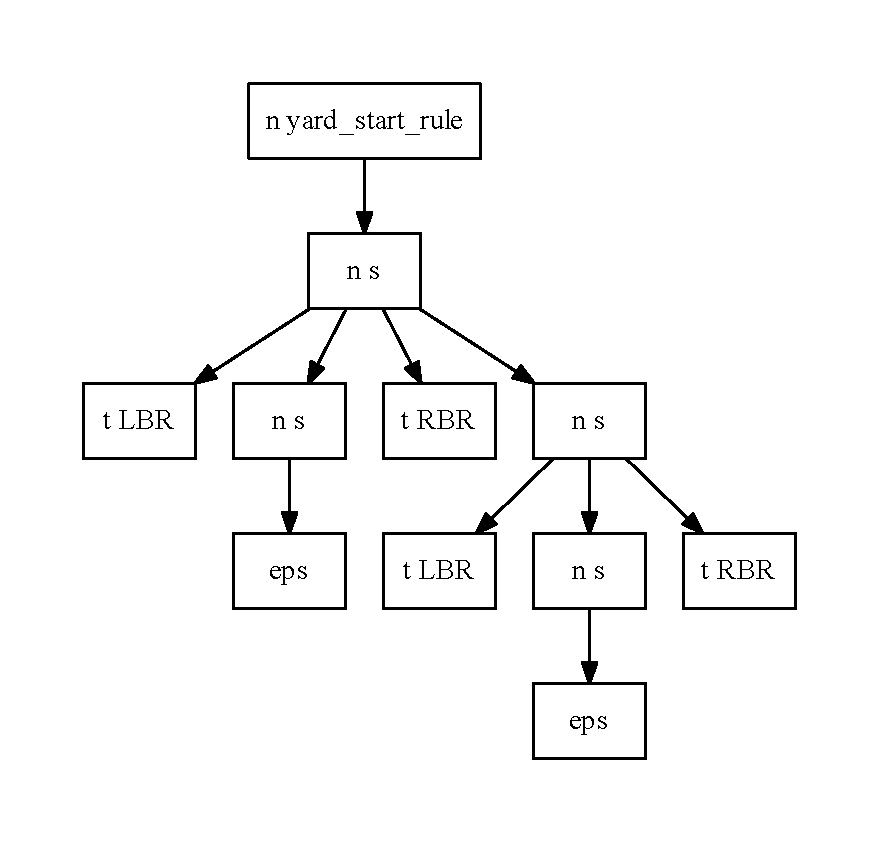
\includegraphics[]{pics/sppf2.pdf}
% \caption{Дерево вывода для выражения $expr="()()"$}
% \label{sppf2}
%\end{figure}
\begin{figure}[!h]
 \centering
 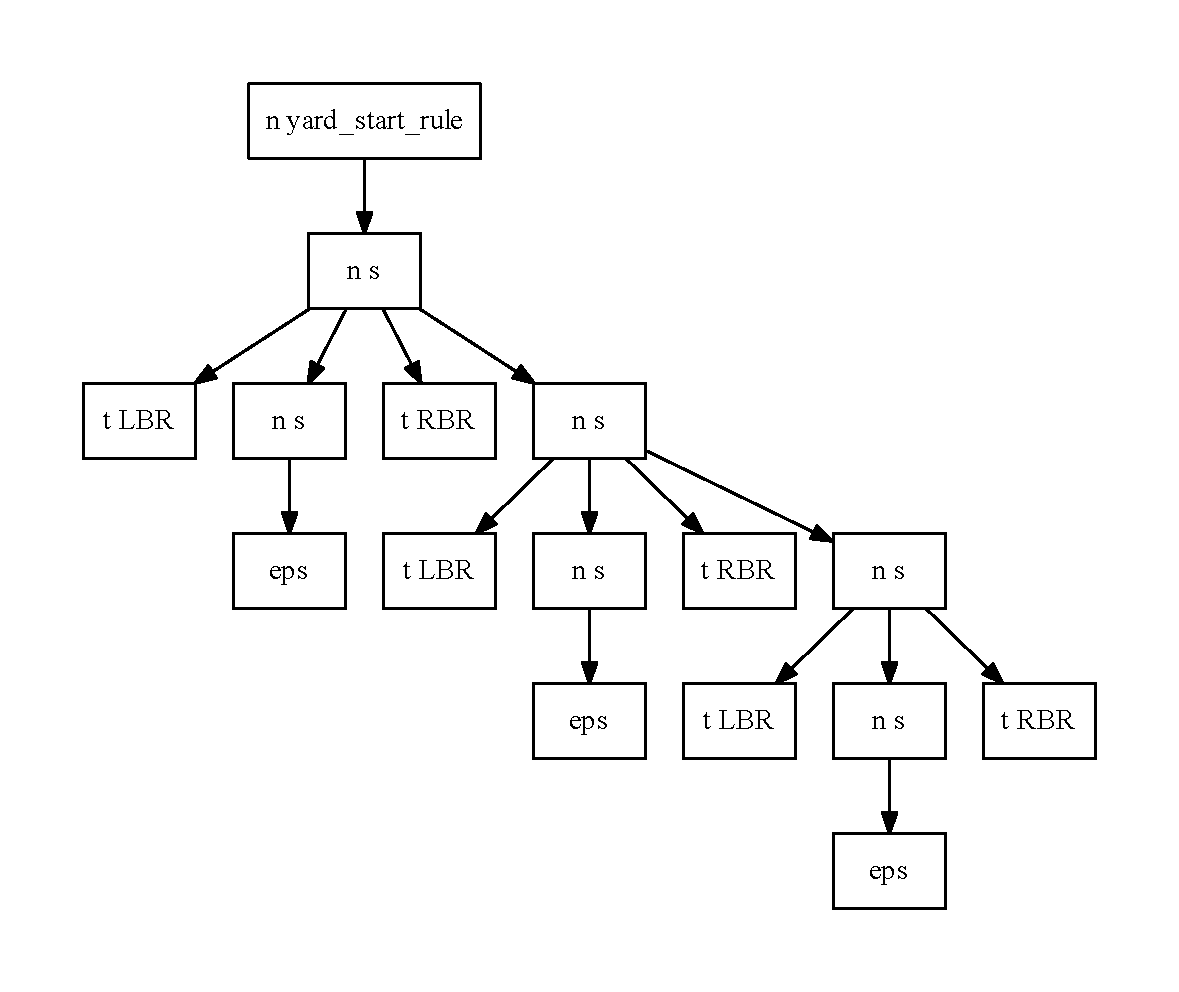
\includegraphics[width=\textwidth]{Verbitskaya/pics/sppf3.pdf}
 \caption{Дерево вывода для выражения $expr="()()()"$}
 \label{sppf3}
\end{figure}

Из SPPF можно извлечь бесконечное количество деревьев, каждое из которых является деревом вывода некоторого выражения из регулярной аппроксимации. Рис.~\ref{sppf3} демонстрирует одно из таких деревьев разбора. 
